%%%%%%%%%%%%%%%%%%%%%%%%%%%%%%%%%%%%%%%%%%%%%%%%%%%%%%%%%%%%%%%%%%%
%                                                                 %
%  GEANT manual in LaTeX form                                     %
%                                                                 %
%  Version 1.00                                                   %
%                                                                 %
%  Last Mod. 8 June 1993  17:20  MG                               %
%                                                                 %
%%%%%%%%%%%%%%%%%%%%%%%%%%%%%%%%%%%%%%%%%%%%%%%%%%%%%%%%%%%%%%%%%%%
\documentstyle[11pt,fleqn,epsfig,crngeant,bibunits,fontcmds,multicol]{cernman}
\newcommand{\Title}{GEANT User's Guide}%           Title for document
\psfigdriver{DVIPS}
\makeindex
\romanfont{times}
\PScommands% Initialize PS boxes
\newmathalphabet*{\mathtt}{cmtt}{m}{n}
\newmathalphabet*{\mathbf}{cmr}{b}{n}
\begin{document}
%  ==================== Front material ============================
%%%%%%%%%%%%%%%%%%%%%%%%%%%%%%%%%%%%%%%%%%%%%%%%%%%%%%%%%%%%%%%%%%%
%                                                                 %
%   GEANT -- Short write ups -- LaTeX Source                      %
%                                                                 %
%   Front Material: Title page,                                   %
%                   Copyright Notice                              %
%                   Preliminary Remarks                           %
%                   Table of Contents                             %
%   EPS file      : cern15.eps, cnastit.eps                       %
%                                                                 %
%   Editor: Michel Goossens / CN-AS                               %
%   Last Mod.: 11 June 1993 10:30 mg                              %
%                                                                 %
%%%%%%%%%%%%%%%%%%%%%%%%%%%%%%%%%%%%%%%%%%%%%%%%%%%%%%%%%%%%%%%%%%%
 
%%%%%%%%%%%%%%%%%%%%%%%%%%%%%%%%%%%%%%%%%%%%%%%%%%%%%%%%%%%%%%%%%%%%
%    Tile page                                                     %
%%%%%%%%%%%%%%%%%%%%%%%%%%%%%%%%%%%%%%%%%%%%%%%%%%%%%%%%%%%%%%%%%%%%
\latex{\def\Ptitle#1{\special{ps: /Printstring (#1) def}
                       \epsfbox{eps/cnastit.eps}}}
 
\begin{titlepage}
%begin{latexonly}
\vspace*{-23mm}%

\includegraphics[height=30mm]{cern.eps}
\hfill
\raise8mm\hbox{\Large\bf CERN Program Library Long Writeup W5013}
\hfill\mbox{}
\begin{center}
\mbox{}\\[6mm]
\mbox{\Ptitle{GEANT}}\\[3cm]
{\Huge Detector Description and}\\[2cm]
{\Huge Simulation Tool}\\[4cm]
{\Large Application Software Group}\\[6mm]
{\Large Computing and Networks Division}\\[2cm]
\end{center}
\vfill
\begin{center}\Large CERN Geneva, Switzerland\end{center}
%end{latexonly}
\begin{htmlonly}
\begin{center}
\Large CERN Program Library Long Writeup W5013\\[1cm]
\Huge GEANT\\[2cm]
\Large Detector Description and Simulation Tool\\[1cm]
\large IT/ASD Group\\
\large CERN, Geneva, Switzerland
\end{center}
\end{htmlonly}
\end{titlepage}

%%%%%%%%%%%%%%%%%%%%%%%%%%%%%%%%%%%%%%%%%%%%%%%%%%%%%%%%%%%%%%%%%%%%
%    Copyright  page                                               %
%%%%%%%%%%%%%%%%%%%%%%%%%%%%%%%%%%%%%%%%%%%%%%%%%%%%%%%%%%%%%%%%%%%%

\thispagestyle{empty}
\framebox[\textwidth][t]{\hfill\begin{minipage}{0.96\textwidth}%
\vspace*{3mm}
\begin{center}Copyright Notice\end{center}
\parskip\baselineskip

\textbf{GEANT -- Detector Description and Simulation Tool}
 
\copyright{} Copyright CERN, Geneva 1993
 
Copyright and any other appropriate legal protection of these
computer programs and associated documentation reserved in all
countries of the world.
 
These programs or documentation may not be reproduced by any
method without prior written consent of the Director-General
of CERN or his delegate.
 
Permission for the usage of any programs described herein is
granted apriori to those scientific institutes associated with
the CERN experimental program or with whom CERN has concluded
a scientific collaboration agreement.
 
CERN welcomes comments concerning the Geant code
but undertakes no obligation for the maintenance of the programs,
nor responsibility for their correctness, and accepts no liability
whatsoever resulting from the use of its programs.
 
Requests for information should be addressed to:
\vspace*{-.5\baselineskip}
\begin{center}\ttfamily
\begin{tabular}{l}
CERN Program Library Office              \\
CERN-IT Division                         \\
CH-1211 Geneva 23                        \\
Switzerland                              \\
Tel.      +41 22 767 4951                \\
Fax.      +41 22 767 7155                \\
Email:    cernlib@cern.ch                \\
WWW:      http://wwwinfo.cern.ch/asd/index.html
\end{tabular}
\end{center}
\vspace*{2mm}
\end{minipage}\hfill}%end of minipage in framebox
\vspace{6mm}
 
{\bf Trademark notice: All trademarks appearing in this guide are acknowledged as such.}
\vfill

\begin{tabular}{l@{\quad}l@{\quad}>{\small\ttfamily}l}
\emph{Contact Persons}:       & IT/ASD/SImulation section & (giani\atsign cern.ch)\\[1mm]
\emph{Documentation Consultant}: & Michel Goossens /IT    & (goossens\atsign cern.ch)\\[1cm]
\textem{Edition -- March 1994}
\end{tabular}
\newpage
 

%  ==================== Body of text ==============================
\pagenumbering{arabic}
\setcounter{page}{1}
 
%%%%%%   Catalog of Program packages and entries%%%%
 
\def\Rtnr{Catalog}%Dummy routine name to appear at bottom of page
%%%%%%%%%%%%%%%%%%%%%%%%%%%%%%%%%%%%%%%%%%%%%%%%%%%%%%%%%%%%%%%%%%%
%                                                                 %
%  GEANT manual in LaTeX form   	                          %
%                                                                 %
%  Michel Goossens (for translation into LaTeX)                   %
%  Version 2.00                                                   %
%  Last Mod.  2 Jun 1998  17:10   MG                              %
%                                                                 %
%%%%%%%%%%%%%%%%%%%%%%%%%%%%%%%%%%%%%%%%%%%%%%%%%%%%%%%%%%%%%%%%%%%
%%% Generated from headings
\chapter{Catalog of Geant sections}
\begin{DLtt}{12345678}
\item[AAAA001] Foreword
\item[AAAA002] Introduction to the manual
\item[BASE001] Introduction to GEANT
\item[BASE010] Simplified Program Flow Chart
\item[BASE020] The data structures and their relationship
\item[BASE040] Summary of Data Records
\item[BASE090] The reference systems and physical units
\item[BASE100] Examples of GEANT application
\item[BASE110] The system initialisation routines
\item[BASE200] Steering routines for event processing
\item[BASE280] Storing and retrieving JRUNG and JHEAD information
\item[BASE299] The banks JRUNG and JHEAD
\item[BASE300] Example of user termination routine
\item[BASE400] Debugging facilities
\item[BASE410] Utility Routines
\item[BASE420] The random number generator
\item[CONS001] Introduction to the section CONS
\item[CONS100] Material definition
\item[CONS101] Retrieve material cross-sections and stopping power
\item[CONS110] Mixtures and Compounds
\item[CONS199] The Material data structure JMATE
\item[CONS200] Tracking medium parameters
\item[CONS210] Special Tracking Parameters
\item[CONS300] Particle definition
\item[CONS310] Branching Ratios and Particle Decay Modes
\item[DRAW001] Introduction to the Drawing package
\item[DRAW010] The Ray-tracing package
\item[DRAW110] Drawing a Volume -- Case 1
\item[DRAW115] Drawing a Volume Projection view -- Case 2
\item[DRAW120] Draw a volume cut view
\item[DRAW130] Draw Particle Trajectories
\item[DRAW140] Drawing Track Hits in Sensitive Detectors
\item[DRAW210] Drawing the geometrical tree
\item[DRAW220] Drawing volume specifications
\item[DRAW300] Handling View banks
\item[DRAW399] The data structure JDRAW
\item[DRAW400] Utility routines of the drawing package
\item[GEOM001] The geometry package
\item[GEOM010] Tracking inside volumes and optimisation
\item[GEOM020] ``MANY'' Volumes and boolean operations on volumes
\item[GEOM050] The GEANT shapes
\item[GEOM100] Creation of a volume
\item[GEOM110] Positioning a volume inside its mother
\item[GEOM120] Positioning a volume inside its mother with parameters
\item[GEOM130] Division of a volume into a given number of cells
\item[GEOM140] Division of a Volume into cells of a given size
\item[GEOM150] Division of a volume - general case
\item[GEOM199] The volume data structure -- JVOLUM
\item[GEOM200] Rotation matrices
\item[GEOM299] The rotation matrix data structure JROTM
\item[GEOM300] Finding in which volume a point is
\item[GEOM310] Finding distance to next boundary
\item[GEOM320] Reference system transformations
\item[GEOM400] Pseudo-division of a volume
\item[GEOM410] Ordering the contents of a volume
\item[GEOM500] Volume attributes
\item[GEOM600] User initialisation of the common block /GCVOLU/
\item[GEOM700] Medium search statistics
\item[GEOM900] End of geometry definition
\item[GEOM910] The CADINT Interface
\item[HITS001] The detector response package
\item[HITS100] Sensitive DETector definition
\item[HITS105] Detector aliases
\item[HITS110] DETector hit parameters
\item[HITS120] DETector Digitisation parameters
\item[HITS130] User detector parameters
\item[HITS199] The SET data structure JSET
\item[HITS200] Routines to store and retrieve HITS
\item[HITS299] The JHITS data structure
\item[HITS300] Routines to store and retrieve DIGItisations
\item[HITS399] The JDIGI data structure
\item[HITS400] Intersection of a track with a cylinder or a plane
\item[HITS500] Digitisation for drift- or MWP- Chambers
\item[HITS510] Digitisation for drift chambers
\item[IOPA001] The I/O routines
\item[IOPA200] ZEBRA sequential files handling
\item[IOPA300] Data structure I/O with sequential files
\item[IOPA400] ZEBRA direct access files handling
\item[IOPA500] Data structure I/O with direct access files
\item[KINE001] Section KINE
\item[KINE100] Storing and retrieving vertex and track parameters
\item[KINE199] The data structures JVERTX and JKINE
\item[KINE200] Interface to the Lund Monte Carlo
\item[KINE210] $\tau ^{\pm }$ generation and decay
\item[PHYS001] Introduction to the section PHYS
\item[PHYS010] Compute the occurrence of a process
\item[PHYS100] Steering routine for physics initialisation
\item[PHYS210] Total cross-section for e+e- pair production by photons
\item[PHYS211] Simulation of e-e+ pair production by photons
\item[PHYS220] Total cross-section for Compton scattering
\item[PHYS221] Simulation of Compton scattering
\item[PHYS230] Total cross-section for photoelectric effect
\item[PHYS231] Simulation of photoelectric Effect
\item[PHYS240] Photon-induced fission on heavy materials
\item[PHYS250] Total cross-section for Rayleigh scattering
\item[PHYS251] Simulation of Rayleigh scattering
\item[PHYS260] \v{C}erenkov photons
\item[PHYS320] Gaussian multiple scattering
\item[PHYS325] Moli\`ere scattering
\item[PHYS328] Plural scattering
\item[PHYS330] Ionisation processes induced by e+/e-
\item[PHYS331] Simulation of the delta-ray production
\item[PHYS332] Simulation of energy loss straggling
\item[PHYS333] Information about energy loss fluctuations
\item[PHYS334] Models for energy loss fluctuations in thin layers
\item[PHYS337] Birks' saturation law
\item[PHYS340] Total cross-section and energy loss for bremsstrahlung by e-e+
\item[PHYS341] Simulation of discrete bremsstrahlung by electrons
\item[PHYS350] Total cross-section for e+e- annihilation
\item[PHYS351] Simulation of e+e- annihilation
\item[PHYS360] Synchrotron radiation
\item[PHYS400] Simulation of particle decays in flight
\item[PHYS410] Rotations and Lorentz transformation
\item[PHYS430] Ionisation processes for muons and protons
\item[PHYS431] Ionisation processes for heavy ions
\item[PHYS440] Total cross-section and energy loss for bremsstrahlung by Muons
\item[PHYS441] Simulation of discrete bremsstrahlung by muons
\item[PHYS450] Total cross-section and energy loss for e-e+ pair production by muons
\item[PHYS451] Simulation of e+e- pair production by muons
\item[PHYS460] Muon-nucleus interactions
\item[PHYS510] The GEANT/GHEISHA Interface
\item[PHYS520] The GEANT/FLUKA Interface
\item[PHYS530] The GEANT/MICAP interface
\item[TRAK001] The tracking package
\item[TRAK110] Steering routine to track one event
\item[TRAK120] Steering routine to track one particle
\item[TRAK130] Tracking one particle through a volume
\item[TRAK200] The tracking routines block diagrams
\item[TRAK300] Storing secondary tracks in the stack
\item[TRAK310] Altering the order of tracking secondary particles
\item[TRAK399] The temporary stack data structure JSTAK
\item[TRAK400] Handling of track space points
\item[TRAK499] The space point data structure JXYZ
\item[TRAK500] Tracking routines in magnetic field
\item[XINT001] The interactive version of GEANT
\item[XINT002] Introduction to the Interactive version of GEANT
\item[XINT010] Screen views of GEANT++
\item[ZZZZ010] List of COMMON Blocks
\item[ZZZZ999] Index of Documented GEANT routines
\end{DLtt}

 
\let\LARGE\large
\let\Large\large
\let\DL\DLtt 

% Here come the different files to be included
 
%%     CONS part     %%
 
\begin{bibunit}[unsrt]
\renewcommand{\bibname}{CONS Bibliography}
\cleardoublepage
%%%%%%%%%%%%%%%%%%%%%%%%%%%%%%%%%%%%%%%%%%%%%%%%%%%%%%%%%%%%%%%%%%%
%                                                                 %
%  GEANT manual in LaTeX form                                     %
%                                                                 %
%  Michel Goossens (for translation into LaTeX)                   %
%  Version 1.00                                                   %
%  Last Mod. Jan 24 1991  1300   MG + IB                          %
%                                                                 %
%%%%%%%%%%%%%%%%%%%%%%%%%%%%%%%%%%%%%%%%%%%%%%%%%%%%%%%%%%%%%%%%%%%
\Documentation{F.Bruyant}   
\Version{Geant 3.16}\Routid{CONS001}
\Submitted{01.10.84}    \Revised{17.12.93}
\Makehead{Introduction to the section CONS}
\section{Introduction}
 
The setup where the particles are transported is represented by a 
structure of geometrical volumes. Each volume is
filled with matter (which can have the properties of the vacuum in case
of it contains no matter).

The matter composing the volumes is described via
two sets of attributes. The first set is relative to the nature
of the {\it material} composing the volume, and contains information
such as the atomic number, the atomic weight, the density and so on
(see the description of the routine \Rind{GSMATE} in this section for
more information). 

The second set of attributes is relevant to the
process of particle transport 
and they define a so-called {\it tracking medium}. These are
parameters such as the material composing the volume,
the magnetic field, the required tracking precision,
the maximum energy that can be lost in one step and so on (see the
description of the routine \Rind{GSTMED} in this section for more
information).

Each tracking medium refers to a material via a {\it material
number} which is assigned by the user. Different tracking media can, with
some limitation, refer to the same material.

Each volume is filled by a tracking medium identified by 
a {\it medium number}.
Different volumes may have the same medium number (see {\tt [GEOM]}).
 
The transport of particles through a
setup ({\tt [TRAK]}) requires access to
data which describe:
\begin{itemize}
\item   the geometry of the setup;
\item   the {\it material} and {\it tracking medium} parameters;
\item   the particle properties.
\end{itemize}
The section {\tt [CONS]} contains the routines
for the storage and retrieval of information related to materials,
tracking media and the particles.

{\bf Important note:} many entities in {\tt GEANT} are user-defined
via a subroutine call. One of the arguments of this subroutine is 
a integer number which identifies the entity. Examples are materials,
tracking media, particles and so on. It can be tempting, for booking
purposes, to use very large numbers. For instance, in a large detector,
the number of all the materials in the hadronic calorimeter could be
$1001 \leq I \leq 2000$. Even if these conventions are very handy, they
can introduce a performance penalty.

For reasons of speed, the number provided by the user is used directly
as the number of the link in the {\tt ZEBRA} data structure indicating
where to store the pointer to
the bank containing the information on the entity. {\tt ZEBRA} 
pointers are contiguous. Defining an object with a user number of $1000$
forces {\tt ZEBRA} to allow space for $1000$ links. This entails a loss
of space ($999$ words), but much worse than that, induces {\tt ZEBRA} to
believe that there are in fact $999$ more banks. At every operation which 
causes a {\it relocation} of banks, {\tt ZEBRA} will check all the possible 
links, which can be very time consuming.

So values of user-defined entities must be kept as small as possible and
contiguous. In large applications one could write a routine which returns
the next free number to be allocated, which can then be stored in a variable
and always referenced symbolically, freeing the user from the need to define
ranges. As an example we give here a function performing this operation
for the material number:
\begin{verbatim}
      FUNCTION NEXTMA()
+SEQ, GCBANK
      IF(JMATE.LE.0) THEN
         NEXTMA = 1
      ELSE
         DO 10 IMAT = 1, IQ(JMATE-2)
            IF(LQ(JMATE-IMAT).EQ.0) GOTO 20
  10     CONTINUE
  20     NEXTMA = IMAT
      ENDIF
      END
\end{verbatim}

\section{Materials}
The material constants are stored in the data structure {\tt JMATE} via the 
routine \Rind{GSMATE} and can be retrieved via the routine \Rind{GFMATE} and 
printed via the routine \Rind{GPMATE}. The routine \Rind{GMATE} calls
repeatedly the routine \Rind{GSMATE} to define a standard set of materials, 
but its use is not mandatory. Mixtures of basic materials, compounds or
molecules with atoms
from different basic materials, may also be defined and their characteristics
are stored in the structure {\tt JMATE}, through calls to the routine
\Rind{GSMIXT}. Mixtures of compounds are allowed.

Quantities such as energy loss and cross-section tables (see {\tt [PHYS]}),
computed during the initialisation of the program are stored in the 
structure {\tt JMATE}. These can be accessed through the routine \Rind{GFTMAT}
and plotted or printed through the routines \Rind{GPLMAT} and \Rind{GPRMAT} 
respectively.

\section{Tracking media}
 
The tracking medium
parameters are stored in the data
structure {\tt JTMED} by the routine \Rind{GSTMED}. Details
about these parameters are given
in {\tt [TRAK]}. They can be accessed with the routine
\Rind{GFTMED} and printed with the routine \Rind{GPTMED}.

The correctness of the transport process and thus the reliability
of the results obtained with {\tt GEANT} depend critically on the
values of the {\it tracking medium parameters}. To help the user,
most of the parameters are recalculated by default by {\tt GEANT}
irrespective of the value assigned by the user. Advanced users
can control the value of the parameters thus bypassing the automatic
computation. See the description of the routine \Rind{GSTMED} for
more information.

The tracking thresholds, and other parameters and flags that control
the physics processes, defined in \Rind{GINIT} and possibly
modified through the relevant data records, are also stored in the structure
{\tt JTMED}. These parameters can be redefined for each tracking medium
via the routine \Rind{GSTPAR}.

\section{Particles}
The parameters of the particles transported by {\tt GEANT}
are stored in the data structure
{\tt JPART} via the routine \Rind{GSPART}. 
The decay properties of particles are defined via the routine \Rind{GSDK}.
The particle constants can be
accessed with the routine \Rind{GFPART} and printed with the routine
\Rind{GPPART}.

The routine \Rind{GPART} defines the standard table of particles,
branching ratios and decay modes. This routine needs to be called for 
the {\tt GEANT} system to work properly. 
\Rind{GPART} calls the routine \Rind{GSPART} for the
particle properties and \Rind{GSDK} for the decays for
each particle in the standard {\tt GEANT} table. 
The user may call \Rind{GSPART} and
\Rind{GSDK} to extend or modify the table defined by \Rind {GPART}.

%%%%%%%%%%%%%%%%%%%%%%%%%%%%%%%%%%%%%%%%%%%%%%%%%%%%%%%%%%%%%%%%%%%
%                                                                 %
%  GEANT manual in LaTeX form                                     %
%                                                                 %
%  Version 1.00                                                   %
%  Last Mod.  8 June 1993 1300   MG                               %
%                                                                 %
%%%%%%%%%%%%%%%%%%%%%%%%%%%%%%%%%%%%%%%%%%%%%%%%%%%%%%%%%%%%%%%%%%%
\Origin{R.Brun, G.N.Patrick} 
\Version{Geant 3.16}\Routid{CONS100}
\Submitted{06.06.83}             \Revised{01.11.93}
\Makehead{Material definition}
\Shubr{GMATE}{}
 
Stores the following standard material constants
in the data structure \cite{bib-PDGD}
{\tt JMATE}.
\begin{center}\begin{tabular}{|l|r|r|r|r|r|}
 \hline
Material   &No. &A         &Z       &Density   &Radiat L   \\
\hline
Hydrogen   &1   &1.010     &1.000   &0.071     &865.000    \\
Deuterium  &2   &2.010     &1.000   &0.162     &757.000    \\
Helium     &3   &4.000     &2.000   &0.125     &755.000    \\
Lithium    &4   &6.940     &3.000   &0.534     &155.000    \\
Beryllium  &5   &9.010     &4.000   &1.848     &35.300     \\
Carbon     &6   &12.010    &6.000   &2.265     &18.8       \\
Nitrogen   &7   &14.010    &7.000   &0.808     &44.500     \\
Neon       &8   &20.180    &10.000  &1.207     &24.000     \\
Aluminium  &9   &26.980    &13.000  &2.700     &8.900      \\
Iron       &10  &55.850    &26.000  &7.870     &1.760      \\
Copper     &11  &63.540    &29.000  &8.960     &1.430      \\
Tungsten   &12  &183.850   &74.000  &19.300    &0.350      \\
Lead       &13  &207.190   &82.000  &11.350    &0.560      \\
Uranium    &14  &238.030   &92.000  &18.950    &0.320      \\
Air        &15  &14.610    &7.300   &$1.205 \times 10^{-3}$ &30423  \\
Vacuum     &16  &$10^{-16}$ &$10^{-16}$ &$10^{-16}$ &$10^{16}$ \\
\hline
\end{tabular} \end{center}
 
{\bf Note:} this table provides some material definition with standard
properties. Advanced user will want to define their own table of materials,
which can be done with the routine \Rind{GSMATE}, described below.
 
\Shubr{GSMATE}{(IMATE,CHNAMA,A,Z,DENS,RADL,ABSL,UBUF,NWBUF)}
Stores the constants for the material {\tt IMATE} in the data structure
{\tt JMATE}.
\begin{DLtt}{MMMMMMMM}
\item[IMATE]      ({\tt INTEGER}) material number;
\item[CHNAMA]     ({\tt CHARACTER*20}) material name;
\item[A]           ({\tt REAL}) atomic weight;
\item[Z]           ({\tt REAL})  atomic number;
\item[DENS]        ({\tt REAL}) density in g cm$^{-3}$;
\item[RADL]        ({\tt REAL}) radiation length in cm;
\item[ABSL]        ({\tt REAL}) absorption length in cm. This parameter
is ignored by {\tt GEANT}, but it has been kept in the calling sequence for
backward compatibility;
\item[UBUF]       ({\tt REAL}) array of {\tt NWBUF} additional user parameters;
\item[NWBUF]      ({\tt INTEGER}) number of user words in {\tt UBUF}.
\end{DLtt}
\Shubr{GFMATE}{(IMATE,CHNAMA*,A*,Z*,DENS*,RADL*,ABSL*,UBUF*,NWBUF*)}
Retrieves the constants of
material {\tt IMATE} from the data structure {\tt JMATE}. The parameters
are the same as for \Rind{GSMATE}.
\Shubr{GPMATE}{(IMATE)}
Prints the material constants:
\begin{DLtt}{MMMMMMMM}
\item[IMATE]   {\tt (INTEGER)} material number. If {\tt IMATE=0} then all
materials will be printed. If {\tt IMATE<0} the material number {\tt -IMATE}
will be printed without the header describing the value of the various fields.
\end{DLtt}

%%%%%%%%%%%%%%%%%%%%%%%%%%%%%%%%%%%%%%%%%%%%%%%%%%%%%%%%%%%%%%%%%%%
%                                                                 %
%  GEANT manual in LaTeX form                                     %
%                                                                 %
%  Michel Goossens (for translation into LaTeX)                   %
%  Version 1.00                                                   %
%  Last Mod. Jan 24 1991  1300   MG + IB                          %
%                                                                 %
%%%%%%%%%%%%%%%%%%%%%%%%%%%%%%%%%%%%%%%%%%%%%%%%%%%%%%%%%%%%%%%%%%%
\Origin{R.Brun, M.Maire}
\Version{Geant 3.16}\Routid{CONS101}
\Submitted{23.04.86}         \Revised{03.11.93}
\Makehead{Retrieve material cross-sections and stopping power}
 
\Shubr{GFTMAT}{(IMATE,IPART,CHMECA,KDIM,TKIN,VALUE*,PCUT*,IXST*)}
 
{\bf Retrieve} and {\bf interpolate} the $dE/dx$ and cross-sections
tabulated in material banks corresponding to a given array of kinetic
energy bins. 

\begin{DLtt}{MMMMMMMM}
\item[IMATE]     ({\tt INTEGER}) material number;
\item[IPART]     ({\tt INTEGER}) particle number;
\item[CHMECA] ({\tt CHARACTER*4}) name of the mechanism bank to be retrieved;
\item[KDIM]  ({\tt INTEGER}) dimension of the arrays {\tt TKIN} and {\tt VALUE};
\item[TKIN]   ({\tt REAL}) array of kinetic energies in GeV;
\item [VALUE]    ({\tt REAL}) array of energy losses in MeV cm$^{-1}$, 
or macroscopic cross sections in cm$^{-1}$;
\item[PCUT]({\tt REAL}) array containing the 5 energy thresholds for the material
in GeV ({\tt CUTGAM}, {\tt CUTELE}, {\tt CUTNEU}, {\tt CUTHAD}, {\tt CUTMUO});
\item[IXST] ({\tt INTEGER}) return code:
\begin{DLtt}{MMM}
\item[0]   the table was not filled:
\item[1]   normal return;
values are returned into the {\tt VALUE} array;
\end{DLtt}
\end{DLtt}

The mechanisms have the following
conventional name and a code number ({\tt IMECA}):
 
\begin{DLtt}{MMMMMMMM}
\item[HADF (~1)] total hadronic interaction cross-section according
to {\tt FLUKA};
\item[INEF (~2)] hadronic inelastic cross-section according
to {\tt FLUKA};
\item[ELAF (~3)] hadronic elastic cross-section according
to {\tt FLUKA};
\item[NULL (~4)] unused;
\item[NULL (~5)] unused;
\item[HADG (~6)] total hadronic interaction cross-section according
to {\tt GHEISHA};
\item[INEG (~7)] hadronic inelastic cross-section according
to {\tt GHEISHA};
\item[ELAG (~8)] hadronic elastic cross-section according
to {\tt GHEISHA};
\item[FISG (~9)] nuclear fission cross-section according
to {\tt GHEISHA};
\item[CAPG (10)] neutron capture cross-section according
to {\tt GHEISHA};
\item[LOSS (11)] stopping power;
\item[PHOT (12)] photoelectric cross-section;
\item[ANNI (13)] positron annihilation cross-section;
\item[COMP (14)] Compton effect cross-section;
\item[BREM (15)] bremsstrahlung cross-section;
\item[PAIR (16)] photon and muon direct- \Pem\Pep pair cross-section;
\item[DRAY (17)] $\delta$-rays cross-section;
\item[PFIS (18)] photo-fission cross-section;
\item[RAYL (19)] Rayleigh scattering cross-section;
\item[MUNU (20)] muon-nuclear interaction cross-section;
\item[RANG (21)] range in cm;
\item[STEP (22)] maximum step in cm.
\end{DLtt}
 
{\bf Note:}
Common \FCind{/GCMULO/} contains an array {\tt ELOW(200)}
(see {\tt [CONS199]})
with {\tt NEK1} kinetic energy values
ranging from {\tt EKMIN} to {\tt EKMAX}. \Rind{GPHYSI} initialises by
default the first 91 locations of {\tt ELOW} with values of energy
from $10^{-5}$ GeV (10 keV) to $10^{4}$ GeV (10 TeV) equally spaced on
logarithmic scale. This can be controlled by the user via the data
record or the interactive command {\tt ERAN} ({\tt [BASE040]}).
{\tt ELOW} can be used as the input argument {\tt TKIN}, e.g.:
\begin{verbatim}
CALL GFTMAT (10, 1,'PHOT',NEK1, ELOW ,VALUE, PCUT, IXST)
\end{verbatim}
will return in array {\tt VALUE} the photoelectric cross-section
in material number 10.

\Shubr{GPLMAT}{(IMATE,IPART,CHMECA,KDIM,TKIN,IDM)}
 
{\bf Plot} and {\bf interpolate} the $dE/dx$ and cross-sections
tabulated in material banks corresponding to a given array of kinetic
energy bins. The mechanisms are the same as the previous routine. 
If the mechanism name is {\tt 'ALL'}, then all the mechanisms will
be plotted.
 
The first five parameters have the same meaning as in the previous routine
and:
\begin{DLtt}{MMMMMMMM}
\item[IDM]({\tt INTEGER}) treatment of the created histogram(s):
\begin{DLtt}{MMM}
\item[$>0$]fill, print, keep histogram(s);
\item[$=0$]fill, print, delete histogram(s);
\item[$<0$]fill, noprint, keep histogram(s).
\end{DLtt}
\end{DLtt}
The result is not returned to the user as is the case in the previous
routine but it is put in an {\tt HBOOK} histogram. The {\tt HBOOK}
package needs to be initialised by the user via the routine \Rind{HLIMIT},
see {\tt [BASE100]} for more information.
The histogram identifier is calculated as: {\tt 10000*IMATE+100*IPART+IMECA}
where {\tt IMECA} is the mechanism code listed above.
 
\Shubr{GPRMAT}{(IMATE,IPART,CHMECA,KDIM,TKIN)}
 
{\bf Print} and {\bf interpolate} the $dE/dx$ and cross-sections
tabulated in material banks corresponding to a given array of kinetic
energy bins. The mechanisms are the same as the previous routine. 
If the mechanism name is {\tt 'ALL'}, then all the mechanisms will
be printed.

The result is printed in the form of a table.
 
The five parameters have the same meaning as in the previous routine.

%%%%%%%%%%%%%%%%%%%%%%%%%%%%%%%%%%%%%%%%%%%%%%%%%%%%%%%%%%%%%%%%%%%
%                                                                 %
%  GEANT manual in LaTeX form                                     %
%                                                                 %
%  Michel Goossens (for translation into LaTeX)                   %
%  Version 1.00                                                   %
%  Last Mod. Jan 24 1991  1300   MG + IB                          %
%                                                                 %
%%%%%%%%%%%%%%%%%%%%%%%%%%%%%%%%%%%%%%%%%%%%%%%%%%%%%%%%%%%%%%%%%%%
\Origin{R.Brun, M.Maire, J.Allison}
\Documentation{M.Maire}
\Version{Geant 3.16}\Routid{CONS110}
\Submitted{01.06.83}          \Revised{08.12.93}
\Makehead{Mixtures and Compounds}
\Shubr{GSMIXT}{(IMATE,NAMATE,A,Z,DENS,NLMAT,WMAT*)}
 
Defines mixture or compound {\tt IMATE} as composed by
{\tt NLMAT} materials defined via
the arrays {\tt A}, {\tt Z} and {\tt WMAT}.
Mixtures of compounds can also be defined.
 
\begin{DLtt}{MMMMMMMMMM}
\item[IMATE]({\tt INTEGER}) user material (mixture) number;
\item[NAMATE]({\tt CHARACTER*20}) mixture name;
\item[A]({\tt REAL}) array of atomic weights;
\item[Z]({\tt REAL}) array of atomic numbers;
\item[DENS]({\tt REAL}) density in g cm$^{-3}$;
\item[NLMAT]({\tt INTEGER}) number of elements in the mixture;
\begin{DLtt}{MMMMM}
\item[$> 0$]{\tt WMAT} contains the proportion
by weights of each material in the mixture;
\item[$< 0$]{\tt WMAT} contains the proportion by number of
atoms of each kind, the content of {\tt WMAT} in output is
changed to contain the relative weights;
\end{DLtt}
\end{DLtt}
 
\subsection*{Method}
For a compound ({\tt NLMAT} $< 0$), the {\it molecular} weight and charge are:
\[
A_{mol} = \sum_i n_i A_i\mbox{\hspace{3cm}} Z_{mol} = \sum_i n_i Z_i
\]
where $n_i$ {\tt = WMAT(I)} is the number of atoms of the i$^{th}$
component of the molecule. In this case the proportion by weight is:
\[
 p_i = \frac{n_i A_i}{A_{mol}}
\]
where $p_i$ {\tt = WMAT(I)} in output.
From the relative weights,
\Rind{GSMIXT} works out the effective atomic weight and atomic number
according to the following formulas:
\[
A_{eff} = \sum_i p_i A_i \mbox{\hspace{3cm}}   Z_{eff} = \sum_i p_i Z_i
\]
which are stored in the {\tt JMATE} data structure {\tt [CONS199]}
together with the radiation length.
 
The radiation length is computed according to the EGS
manual \cite{bib-EGS3}, formula 268 (37), for an element:
\[
\frac{1} {\rho \: X_0 }=4 \alpha r_{0}^2 N_{Av}  \frac{1}{A}
     Z(Z+ \xi (Z)) \left[ \ln \frac{183}{Z^{1/3}}
      -F_c (Z) \right]
\]
where
\begin{DLtt}{MMMMMMMM}
\item[$X_0$]   radiation length (in cm);
\item[$\rho$] density (in g cm$^{-3}$);
\item[$\alpha$] fine structure constant;
\item[$r$]classical electron radius (in cm);
\item[$N_{Av}$] Avogadro's number;
\item[$A$]atomic weight;
\item[$Z$]atomic number;
\item[$F_c(Z)$] Coulomb correction function.
\end{DLtt}
\[
F_c (Z) = (\alpha Z)^2 \left[ \frac{1}
     { 1+( \alpha Z)^2}  +0.20206-0.0369( \alpha Z)^2
      +0.0083(\alpha Z)^4 -0.0020(\alpha Z)^6 \right]
\]
\[
\xi (Z) = \frac{\ln \frac{1440}{Z^{2/3}}}
        {\ln \frac{183}{Z^{1/3}} - F_c (Z)}
\]
for a compound or mixture:
\[
 \frac{1}{\rho X_0}=\sum_i \frac{p_i}{\rho_i X_{0i}}
\]
where $p_i$ is the proportion by weight of the i$^{th}$ element.
For more information on the organisation of the data in memory
see {\tt [CONS199]}.

The effective absorption length $\lambda$ is defined as
the interaction length of a 5GeV pion in the material:
\[
\frac{1}{\lambda} = \sum_i \frac{p_i}{\lambda_i}
\hspace{2cm} \frac{1}{\lambda_i} = \frac{\sigma^{\pi}_{i}(5GeV)
 N_{Av}}{A_{i}} 
\hspace{0.5cm} \mbox{g$^{-1}$ cm$^{2}$}
\]
Once this value has been determined, an effective hadronic atomic weight 
($A_{h-eff}$) is calculated by the routine \Rind{GHMIX} \cite{bib-GHMI}
and stored in the data structure.

%%%%%%%%%%%%%%%%%%%%%%%%%%%%%%%%%%%%%%%%%%%%%%%%%%%%%%%%%%%%%%%%%%%
%                                                                 %
%  GEANT manual in LaTeX form                                     %
%                                                                 %
%  Michel Goossens (for translation into LaTeX)                   %
%  Version 1.00                                                   %
%  Last Mod. Jan 24 1991  1300   MG + IB                          %
%                                                                 %
%%%%%%%%%%%%%%%%%%%%%%%%%%%%%%%%%%%%%%%%%%%%%%%%%%%%%%%%%%%%%%%%%%%
\Origin{R.Brun}
\Documentation{R.Brun, M.Maire}
\Version{Geant 3.16}\Routid{CONS199}
\Submitted{01.06.83}             \Revised{23.03.94}
\Makehead{The Material data structure JMATE}

\begin{figure}[hbt]
      \centering
      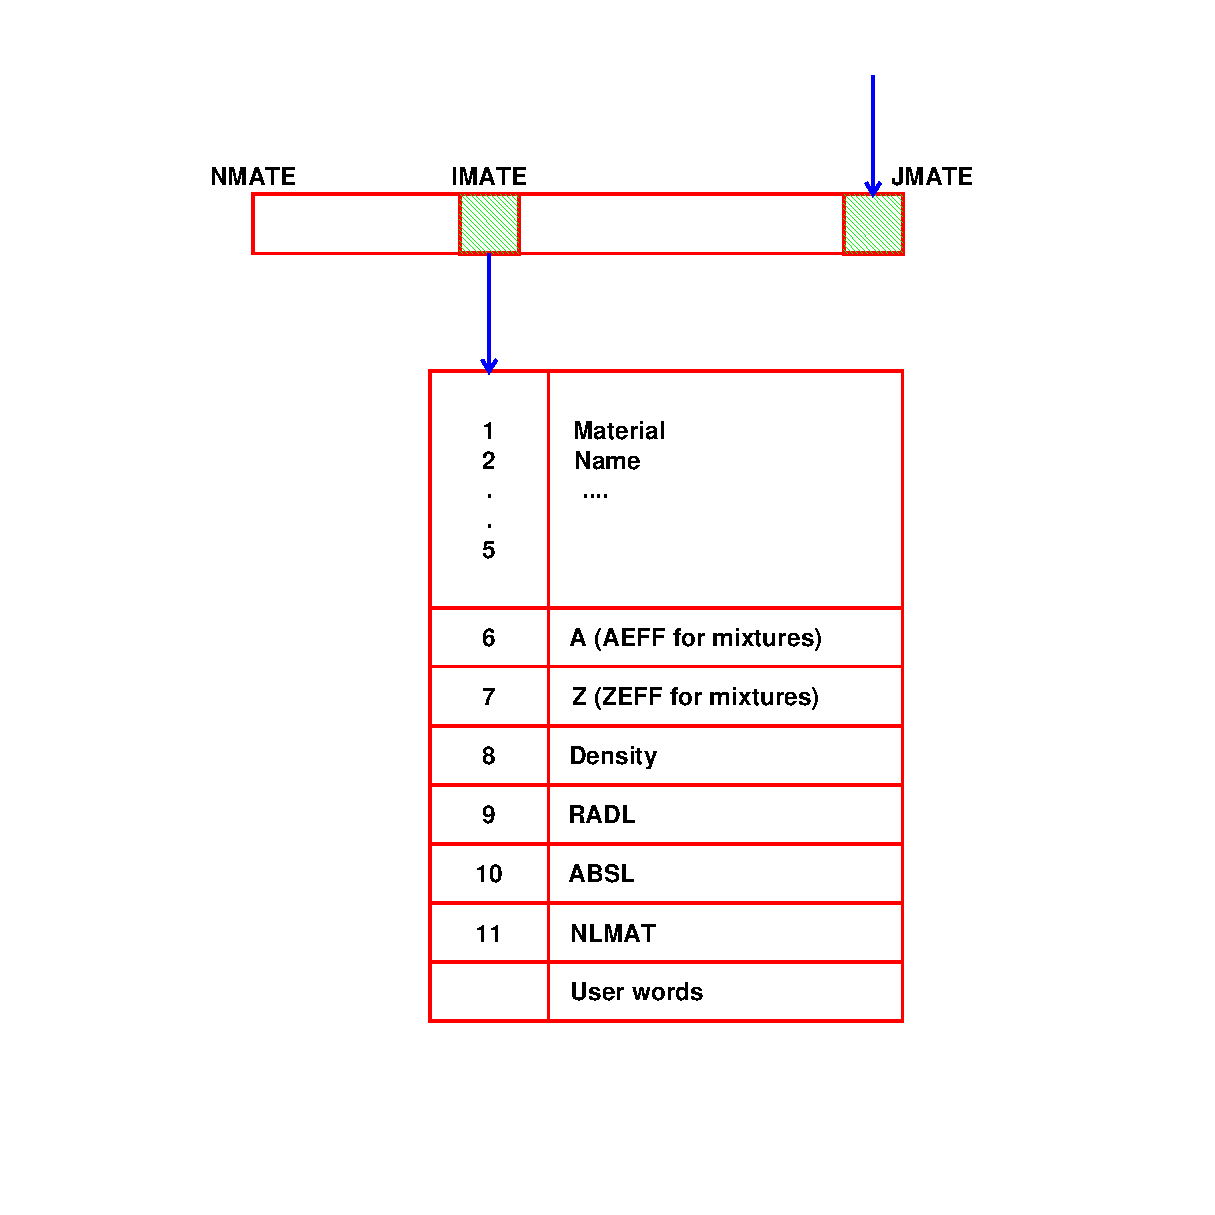
\epsfig{file=eps/cons199-1.eps,width=\linewidth}
      \caption{{\tt JMA = LQ(JMATE-IMATE)} pointer to material {\tt IMATE}}
      \label{cons199-1}
\end{figure}

When the subroutine GPHYSI is called at initialisation time the
following substructure is created for each material whose number
is refered to by any of the user defined tracking media.

\begin{figure}[p]
      \centering
      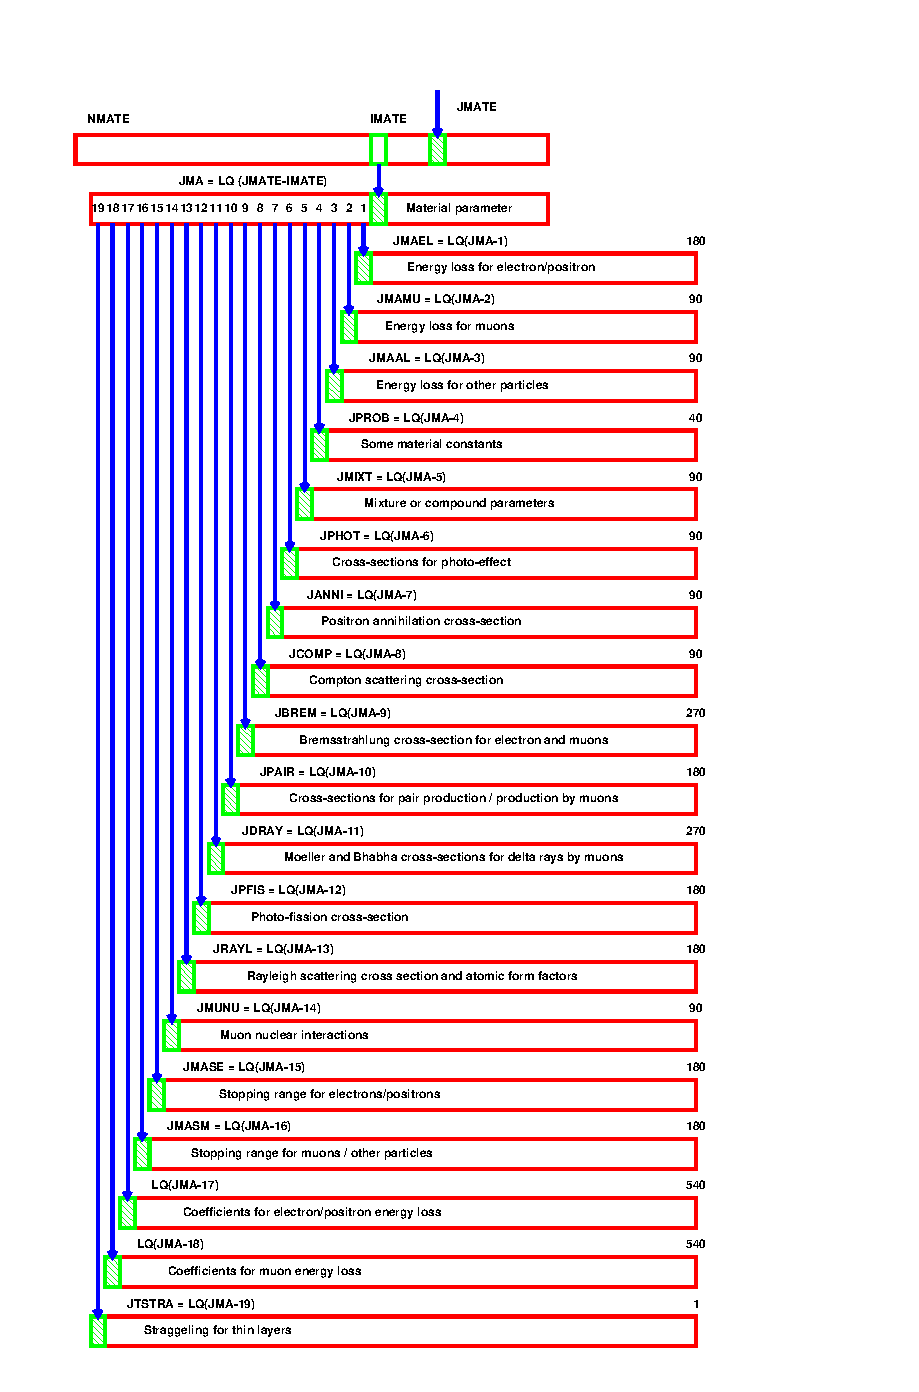
\epsfig{file=eps/cons199-2.eps,height=.95\textheight}
      \caption{Material data structure}
      \label{cons199-2}
\end{figure}

{\bf Note:}
The energy losses are stored in ${\rm GeV \: cm^{-1}}$. The inverse of
the macroscopic cross-section (i.e. the mean free path, in cm), is stored
instead of the cross-section, to speed up the calculation of the distance
to the next interaction point.
 
\section{Energy binning}
 
\begin{center}
\begin{tabular}{|c|l|l|}
\hline
IDECAD  &Bin number  &Energy range \\
& &IEKBIN    \\
\hline
 
1  &1 $\rightarrow$ 10  &10 KeV $\rightarrow$ 79.43 KeV          \\
2  &11 $\rightarrow$ 20  &100 KeV $\rightarrow$ 794.3 KeV       \\
3  &21 $\rightarrow$ 30  &1 MeV $\rightarrow$ 7.943 MeV           \\
4  &31 $\rightarrow$ 40  &10 MeV $\rightarrow$ 79.43 MeV         \\
5  &41 $\rightarrow$ 50  &100 MeV $\rightarrow$ 794.3 MeV       \\
6  &51 $\rightarrow$ 60  &1 GeV $\rightarrow$ 7.943 GeV           \\
7  &61 $\rightarrow$ 70  &10 GeV $\rightarrow$ 79.43 GeV         \\
8  &71 $\rightarrow$ 80  &100 GeV $\rightarrow$ 794.3 GeV       \\
9  &81 $\rightarrow$ 90  &1 TeV $\rightarrow$ 7.943 TeV           \\
\hline
\end{tabular}
\end{center}
 
The values of the bins are kept in the array ELOW(90) in /GCMULO/ :
 
\[
 \mbox{ELOW}(i) = 10 ^ { \frac{i-1}{10} - 5 } [ \mbox{GeV} ]
\]
 
\section{Energy loss for electrons and positrons}
 
Words 1 to 90, for electrons:  DE/DX = Ionisation (Moller) +brems.
 
Words 91 to 180, for positrons:  DE/DX = Ionisation (Bhabha) +brems.
[PHYS 330, 340].
 
\section{Energy loss for muons}
 
  DE/DX = Ionisation +brems. +Direct \Pep\Pem production +Nuclear interacti     on
[PHYS 430, 440, 450].
 
\section{Energy loss for other charged particles}
 
  DE/DX = Ionisation
 
The values are computed for a proton (mass Mp). For any other
particle with mass M and kinetic energy T,
one has to compute the equivalent proton kinetic energy as T*Mp/M
and look at the corresponding energy binning [PHYS 430].
 
\section{Some material constants}
 
Various constants which are material dependent and needed to compute the
cross-sections.
 
See routine GPROBI.
 
\section{Mixture and compound parameters}
 
Words 1 to 4*NLM  where  NLM is the number of mixture or compound
components [CONS110].
 
\section{Photo-electric effect. Muon nuclear interaction}
 
As the photo-electric effect vanishes at high energies
whereas the muon nuclear
interaction cross-section is null at low energies, the two effects are
stored within the same bank in order to save space.
 
From 10 KeV to 50 MeV : Photo-electric effect mean free path [PHYS 230]
From 1 GeV to 10 TeV : Muon nuclear interaction mean free path
[PHYS 460].
 
\section{Positron annihilation}
 
[PHYS 350].
 
\section{Compton scattering}
 
[PHYS 220].
 
\section{Bremsstrahlung for electrons and muons}
 
Words 1 to 90, mean free path for electrons [PHYS 340]
Words 91 to 180, mean free path for muons [PHYS 440].
 
\section{Pair production by gammas and muons}
 
Words 1 to 90, for gammas [PHYS 210].
Words 91 to 180, for muons [PHYS 450].
 
\section{Delta ray production by electrons and muons}
 
Words 1 to 90, for \Pem\Pem $\rightarrow$ \Pem\Pem [PHYS 330].
 
Words 91 to 180, for \Pep\Pem $\rightarrow$ \Pep\Pem [PHYS 330]
 
Words 181 to 270, for \Pem $\rightarrow$ \Pem [PHYS 430].
 
\section{Photo-fission}
 
Only for material with atomic number A>200 [PHYS 240].
%\end{document}
 
 

%%%%%%%%%%%%%%%%%%%%%%%%%%%%%%%%%%%%%%%%%%%%%%%%%%%%%%%%%%%%%%%%%%%
%                                                                 %
%  GEANT manual in LaTeX form                                     %
%                                                                 %
%  Version 1.00                                                   %
%                                                                 %
%  Last Mod. 12 June 1993 1700   MG                               %
%                                                                 %
%%%%%%%%%%%%%%%%%%%%%%%%%%%%%%%%%%%%%%%%%%%%%%%%%%%%%%%%%%%%%%%%%%%
\Origin{R.Brun}            
\Revision{F.Carminati, M.Maire}
\Version{Geant 3.16}           \Routid{CONS200}
\Submitted{01.06.83}           \Revised{08.12.93}
\Makehead{Tracking medium parameters}
\section*{Description of the routines}
\Shubr{GSTMED}{(ITMED,NATMED,NMAT,ISVOL,IFIELD,FIELDM,TMAXFD,STEMAX,
                DEEMAX,EPSIL,STMIN,UBUF,NWBUF)}
This routine associates a set of tracking parameters to a material, defining
a so-called {\it tracking medium}. Every {\tt GEANT} volume must be 
associated to an existing tracking medium. The routine
stores the parameters of the tracking
medium {\tt ITMED} in the data structure {\tt JTMED}.
\begin{DLtt}{MMMMMMMM}
\item[ITMED]      ({\tt INTEGER}) tracking medium number;
\item[NATMED]     ({\tt CHARACTER*20}) tracking medium name;
\item[NMAT]       ({\tt INTEGER}) material number corresponding to {\tt ITMED};
\item[ISVOL]      ({\tt INTEGER}) {\it sensitivity} flag (see later):
\begin{DLtt}{MMMM}
\item[$\leq$0] not a sensitive volume;
\item[$>$0] sensitive volume;
\end{DLtt}
\item[IFIELD]     ({\tt INTEGER}) magnetic field flag:
\begin{DLtt}{MMMM}
\item[=0]         no magnetic field;
\item[=1]         strongly 
inhomogeneous magnetic field (returned by the user function
\Rind{GUFLD}): tracking performed with the Runge-Kutta method by the
routine \Rind{GRKUTA};
\item[=2]         inhomogeneous magnetic field (returned by the user function
\Rind{GUFLD}), tracking along a helix performed by the routine \Rind{GHELIX};
\item[=3]         uniform magnetic field along the {\tt z} axis of strength
{\tt FIELDM}, tracking performed along a helix by the routine \Rind{GHELX3};
\end{DLtt}
\item[FIELDM]     ({\tt REAL}) maximum field value (in Kilogauss);
\item[TMAXFD]     ({\tt REAL}) maximum angular deviation due to the magnetic
field permitted in one step (in degrees);
\item[STEMAX]     ({\tt REAL}) maximum step permitted (cm);
\item[DEEMAX]     ({\tt REAL}) maximum fractional energy loss in one step ($0<$
                  {\tt DEEMAX} $\leq 1$);
\item[EPSIL]      ({\tt REAL}) boundary crossing precision (cm);
\item[STMIN]      ({\tt REAL}) minimum value for the maximum step imposed by 
energy loss, multiple scattering, \v{C}erenkov or magnetic field effects (cm);
\item[UBUF]       ({\tt REAL}) array of {\tt NWBUF} additional user parameters;
\item[NWBUF]      ({\tt INTEGER}) number of additional user parameters.
\end{DLtt}
 
{\bf Note:} the tracking medium number can in principle be any positive
integer from 1 to 65,535. However this number is used directly by {\tt GEANT}
as the number of the pointer to the data structure where the information
is stored. When a pointer is defined,
all pointers from 1 to the one allocated are created, if not already existing.
Every time data structures are moved in memory, all the
links are potentially scanned for update. This can be time consuming and
it can seriously affect performances. So a continuous
range of numbers should be used for tracking media.

\Shubr{GFTMED}{(ITMED,NATMED*,NMAT*,ISVOL*,IFIELD*,FIELDM*,TMAXFD*,
                STEMAX*,DEEMAX*,EPSIL*,STMIN*,UBUF*,NWBUF*)}
 
Extracts the parameters of the tracking medium {\tt ITMED}
from the data structure {\tt JTMED}.
 
\Shubr{GPTMED}{(ITMED)}
 
Prints the tracking medium parameters for the given medium.
\begin{DLtt}{MMMMM}
\item[ITMED]      ({\tt INTEGER}) tracking medium to be printed,
all tracking media if {\tt ITMED}=0.
\end{DLtt}

\section*{Automatic calculation of the tracking parameters}

The results of the simulation depend critically on the choice of the tracking
medium parameters. To make of {\tt GEANT} a reliable and consistent predictive
tool, the calculation of these parameters has been automated.
In a normal GEANT run, the variable {\tt IGAUTO} in common
\FCind{/GCTRAK/} is set to 1. In this case the following parameters 
are calculated by the program:
\begin{eqnarray*}
\mbox{\tt TMAXFD} & = & \left\{
\begin{array}{LL}
20^{\circ} & \mbox{if {\tt TMAXFD} $\leq 0$ or {\tt TMAXFD} $ > 20$} \\
\mbox{\it input value} & \mbox{if $0 <$ {\tt TMAXFD} $\leq 20$}
\end{array} \right . \\
\mbox{\tt STEMAX} & = & \phantom{\{} 
\begin{array}{LL} \mbox{\tt BIG} (=10^{10}) \end{array} \\
\mbox{\tt DEEMAX} & = & \left \{
\begin{array}{LL}
0.25 & \parbox[t]{10cm}{if {\tt ISVOL} $= 0$ and $X_{0} \leq 2cm$, 
where $X_{0}$ is the radiation length of the material} \\
0.25-\frac{0.2}{\sqrt{X_{0}}} & \mbox{otherwise}
\end{array} \right . \\
\mbox{\tt STMIN} & = & \left\{
\begin{array}{LL}
\frac{2 R}{\sqrt{X_{0}}} & \mbox{if {\tt ISVOL} $=0$} \\ [.2cm]
\frac{5 R}{\sqrt{X_{0}}} & \mbox{if {\tt ISVOL} $\neq 0$}
\end{array} \right . 
\end{eqnarray*}

where $R$ is the range in cm of an electron of energy {\tt CUTELE}+200keV.

If the {\tt IGAUTO} variable is set to 0 via the {\tt AUTO} data record, 
then value given by the user for the above parameters is accepted as the
true parameter value if $>0$, while automatic calculation still takes place
in case the input value is negative.

Users are strongly recommended to begin their simulation with the parameters
as calculated by {\tt GEANT}. Users who want to modify any of the above
parameters must be sure they understand their function in the program and
the implications of a change.

The {\tt EPSIL} parameter represents the absolute precision with which the
tracking is performed. It has a double meaning. When tracking in magnetic
field, {\tt EPSIL} is the minimum distance for which boundaries are
checked. A particle nearer than {\tt EPSIL} to the boundary is considered
as exiting the current volume. If the end point of the step of a particle in
magnetic field is distant less than {\tt EPSIL} along each axis 
from what would be the end point in absence of magnetic field, then no boundary 
checking is performed. 

In all cases, when a particle is going to reach the
boundary of the current volume with the current step, the step length is 
increased by a quantity ({\tt PREC}, common \FCind{/GCTMED/}) which is set to the 
minimum between $0.1 \times {\tt EPSIL}$
and 10 micron at the beginning of the tracking. This quantity is recalculated
at every step according to the formula:
\begin{equation}
\mbox{\tt PREC} 
=\max \left [ \min \left(\frac{\mbox{\tt EPSIL}}{10}, 10 \mu \right ) ,
\max \left [ | x |, | y |, | z |, S \right ) \times \epsilon \right ]
\end{equation}
Where $x, y, z$ are the current coordinates of the particle, $S$ is the length
of the track, and $\epsilon$ is the assumed machine precision.
$\epsilon$ (called {\tt EPSMAC} in the program) is initially set to
$10^{-6}$ for 32 bits machines and $10^{-11}$ for 64 bits machines.
During the tracking, every fifth time that a particle tries unsuccessfully
to exit from the same volume, the machine precision is multiplied by the
number of trials. This accounts for additional losses of precision due to
transformation of coordinates and region of the floating point range where
the real machine precision is different from the above (this happens 
in particular on IBM mainframes with 370 floating point number representation).

%%%%%%%%%%%%%%%%%%%%%%%%%%%%%%%%%%%%%%%%%%%%%%%%%%%%%%%%%%%%%%%%%%%
%                                                                 %
%  GEANT manual in LaTeX form                                     %
%                                                                 %
%  Michel Goossens (for translation into LaTeX)                   %
%  Version 1.00                                                   %
%  Last Mod. Jan 24 1991  1300   MG + IB                          %
%                                                                 %
%%%%%%%%%%%%%%%%%%%%%%%%%%%%%%%%%%%%%%%%%%%%%%%%%%%%%%%%%%%%%%%%%%%
\Origin{R.Brun,F.Bruyant}
\Documentation{same}
\Version{Geant 3.16}\Routid{CONS210}
\Submitted{11.02.86}     \Revised{08.12.93}
\Makehead{Special Tracking  Parameters}
 
\Shubr{GSTPAR}{(ITMED,CHPAR,PARVAL)}
 
\begin{DLtt}{MMMMMMMMMM}
\item[ITMED]   ({\tt INTEGER}) tracking medium number;
\item[CHPAR]   ({\tt CHARACTER*4}) character string, name of the variable 
to be modified;
\item[PARVAL]  ({\tt REAL}) new value (must be given as a floating point).
\end{DLtt}
\begin{center} 
\begin{tabular}{|>{\ttfamily}r@{}>{\ttfamily}r@{\quad=\quad}>{\ttfamily}l|>{\ttfamily}l|l|}
 \hline
\multicolumn{3}{|c|}{Default parameters}
& \multicolumn{1}{c|}{Parameter name} 
& \multicolumn{1}{c|}{Default value} \\
\hline
Q(JTMN & +1) & CUTGAM & CUTGAM & 0.001GeV \\
Q(JTMN & +2) & CUTELE & CUTELE & 0.001GeV \\
Q(JTMN & +3) & CUTNEU & CUTNEU & 0.01GeV  \\
Q(JTMN & +4) & CUTHAD & CUTHAD & 0.01GeV  \\
Q(JTMN & +5) & CUTMUO & CUTMUO & 0.01GeV  \\
Q(JTMN & +6) & BCUTE  & BCUTE  & \texttt{CUTGAM}   \\
Q(JTMN & +7) & BCUTM  & BCUTM  & \texttt{CUTGAM}   \\
Q(JTMN & +8) & DCUTE  & DCUTE  & 10.TeV   \\
Q(JTMN & +9) & DCUTM  & DCUTM  & 10.TeV   \\
Q(JTMN & +10)& PPCUTM & PPCUTM & 0.01GeV  \\
Q(JTMN & +11)& IPAIR  &  PAIR  & 1        \\
Q(JTMN & +12)& ICOMP  &  COMP  & 1        \\
Q(JTMN & +13)& IPHOT  &  PHOT  & 1        \\
Q(JTMN & +14)& IPFIS  &  PFIS  & 0        \\
Q(JTMN & +15)& IDRAY  &  DRAY  & 2        \\
Q(JTMN & +16)& IANNI  &  ANNI  & 1        \\
Q(JTMN & +17)& IBREM  &  BREM  & 1        \\
Q(JTMN & +18)& IHADR  &  HADR  & 1        \\
Q(JTMN & +19)& IMUNU  &  MUNU  & 0        \\
Q(JTMN & +20)& IDCAY  &  DCAY  & 1        \\
Q(JTMN & +21)& ILOSS  &  LOSS  & 2        \\
Q(JTMN & +22)& IMULS  &  MULS  & 1        \\
Q(JTMN & +26)& GHEISHA   & GHCOR1 & see \texttt{[PHYS700]}  \\
Q(JTMN & +27)& MODEL     & BIRK1  & see \texttt{[PHYS337]}  \\
Q(JTMN & +28)& RKB     & BIRK2  & see \texttt{[PHYS337]}  \\
Q(JTMN & +29)& C     & BIRK3  & see \texttt{[PHYS337]}  \\
Q(JTMN & +31)& ILABS  & LABS  & see \texttt{[PHYS260]}  \\
Q(JTMN & +32)& ISYNC  & SYNC  & see \texttt{[PHYS360]}  \\
Q(JTMN & +33)& ISTRA  & STRA  & see \texttt{[PHYS333]} \\
\hline
\end{tabular}
\end{center} 
 
The data structure \texttt{JTMED} contains the standard tracking parameters
(\texttt{CUTS} and flags to control the physics processes) which are used by
default for all tracking media. It is possible to redefine individually
with \Rind{GSTPAR} any of these parameters for a given tracking medium.
For example to change \texttt{CUTGAM} to 0.0001 for tracking medium \texttt{ITMED}:
\begin{center}
 \texttt{CALL GSTPAR(ITMED,'CUTGAM',0.0001)}
\end{center}

For more information on default values for \texttt{IDRAY} and \texttt{ILOSS} see
\texttt{[BASE040]}.
 
The default tracking medium parameters are stored in the bank whose
pointer is stored in the \texttt{JTMED} variable. In this case in the
above table \texttt{JTMN} = \texttt{JTMED}. In the case one or more of
the above parameters has been modified for a specific tracking
medium, the whole parameter set is stored in the next bank of the
given trackin medium. In this case \texttt{JTMN} = \texttt{LQ(JTM)} in
the above table, where \texttt{JTM} is the pointer to the bank of the
tracking medium, i.e. \texttt{JTM} = \texttt{LQ(JTMED-ITMED)}.
 
{\bf Note}
 
At tracking time the parameters above are copied
from \texttt{JTMN} into the common blocks
\FCind{/GCCUTS/} and \FCind{/GCPHYS/}. \Rind{GSTPAR} must be called before
\Rind{GPHYSI}.
%\end{document}
 

%%%%%%%%%%%%%%%%%%%%%%%%%%%%%%%%%%%%%%%%%%%%%%%%%%%%%%%%%%%%%%%%%%%
%                                                                 %
%  GEANT manual in LaTeX form                                     %
%                                                                 %
%  Michel Goossens (for translation into LaTeX)                   %
%  Version 1.00                                                   %
%  Last Mod. Jan 24 1991  1300   MG + IB                          %
%                                                                 %
%%%%%%%%%%%%%%%%%%%%%%%%%%%%%%%%%%%%%%%%%%%%%%%%%%%%%%%%%%%%%%%%%%%
\Origin{R.Brun, G.N.Patrick}
\Version{Geant 3.15}\Routid{CONS300}
\Submitted{01.06.83}               \Revised{13.05.92}
\Makehead{Particle definition}
 
\Shubr{GPART}{}
 
Stores the standard particle constants in the data structure
{\tt JPART} and, through the routine \Rind{GSDK}, their decay modes 
{\tt [CONS310]}.
 
\begin{center}
\begin{tabular}{|l|r|l|r|r@{}l|}
\hline
\makebox[2.5cm][l]{Particle} & No.  & 
\makebox[3.2cm][l]{Mass(GeV)} &   Charge & 
\makebox[2.3cm][l]{Life time(sec)} & 
\makebox[1.3cm]{}  \\
\hline
Gamma        & 1 &0.0           &  0 & stable & \hspace{.2cm} ($10^{15}$) \\
Positron     & 2 &0.00051099906 &  1 &  stable &          \\
Electron     & 3 &0.00051099906 & -1 &  stable &          \\
Neutrino     & 4 & 0.0          &  0 &  stable &          \\
Muon +       & 5 &0.105658389   &  1 & $2.19703 $ & $\: \times 10^{-6}$\\
Muon -       & 6 &0.105658389   & -1 & $2.19703 $ & $\: \times 10^{-6}$  \\
Pion 0       & 7 &0.1349764     &  0 & $8.4 $ & $\: \times 10^{-17}$     \\
Pion +       & 8 &0.1395700     &  1 & $2.603 $ & $\: \times 10^{-8}$   \\
Pion -       & 9 &0.1395700     & -1 & $2.603 $ & $\: \times 10^{-8} $  \\
Kaon 0 long  &10 &0.497672      &  0 & $5.17 $ & $\: \times  10^{-8}$    \\
Kaon +       &11 &0.493677      &  1 & $1.237 $ & $\: \times 10^{-8}$   \\
Kaon -       &12 &0.493677      & -1 & $1.237 $ & $\: \times 10^{-8}$    \\
Neutron      &13 &0.93956563    &  0 & $  887.0 $ &                 \\
Proton       &14 &0.93827231    &  1 & stable    &         \\
Antiproton   &15 &0.93827231    & -1 & stable    &         \\
Kaon 0 short &16 &0.497672      &  0 & $ 8.926 $ & $\: \times 10^{-11}$   \\
Eta          &17 &0.54745       &  0 & $ 5.485   $ & $\: \times 10^{-19}$ \\
Lambda       &18 &1.115684      &  0  & $ 2.632 $ & $\: \times 10^{-10}$    \\
Sigma +      &19 &1.18937       &  1  & $ 7.99   $ & $\: \times 10^{-11}$     \\
Sigma 0      &20 &1.19255       &  0  & $ 7.40 $ & $\: \times  10^{-20}$   \\
Sigma -      &21 &1.197436      & -1  & $1.479 $ & $\: \times  10^{-10}$   \\
Xi 0         &22 &1.3149        &  0  & $2.90 $ & $\: \times  10^{-10}$   \\
Xi -         &23 &1.32132       & -1  & $1.639 $ & $\: \times 10^{-10}$   \\
Omega        &24 &1.67245       & -1  & $ 8.22 $ & $\: \times 10^{-11}$   \\
Antineutron  &25 &0.93956563    &  0  & $ 887.0 $  &           \\
Antilambda   &26 &1.115684      &  0  &  $ 2.632 $ & $\: \times 10^{-10}$  \\
Antisigma -  &27 &1.18937       & -1  &  $ 7.99 $ & $\: \times 10^{-11}$   \\
Antisigma 0  &28 &1.19255       &  0  &  $ 7.40 $ & $\: \times  10^{-20}$   \\
Antisigma +  &29 &1.197436      &  1  &  $ 1.479 $ & $\: \times 10^{-10}$   \\
Antixi 0     &30 &1.3149        &  0  &  $ 2.90 $ & $\: \times   10^{-10}$   \\
Antixi +     &31 &1.32132       &  1  &  $ 1.639 $ & $\: \times 10^{-10}$  \\
\hline
\end{tabular}
\end{center}
\newpage
\begin{center}
\begin{tabular}{|l|r|l|r|r@{}l|}
\hline
\makebox[2.5cm][l]{Particle} & No.  & 
\makebox[3.2cm][l]{Mass(GeV)} &   Charge & 
\makebox[2.3cm][l]{Life time(sec)} & 
\makebox[1.3cm]{}  \\
\hline
Antiomega +  &32    &1.67245    &   1     &  $ 8.22 $ & $\: \times  10^{-11}$  \\
%Tau +      &33    &1.7841     &   1     &  $ 3.04 $ & $\: \times 10^{-13}$   \\
%Tau -      &34    &1.7841     &   1     &  $ 3.04 $ & $\: \times 10^{-13}$  \\
%D+         &35    &1.8693     &   1     &  $ 1.062 $ & $\: \times 10^{-12}$  \\
%D-         &36    & 1.8693    &  -1     &  $ 1.062 $ & $\: \times 10^{-12}$  \\
%D0         &37    & 1.8645    &   0     &  $ 4.28 $ & $\: \times 10^{-13}$  \\
%Anti D0    &38    & 1.8645    &   0     &  $4.28 $ & $\: \times  10^{-13}$   \\
%DS+        &39    & 1.9693    &   1     &  $ 4.36 $ & $\: \times 10^{-13}$   \\
%DS-        &40    & 1.9693    &  -1     &  $ 4.36 $ & $\: \times 10^{-13}$   \\
%Lambda C+  &41    & 2.2849    &   1     &  $ 1.79 $ & $\: \times 10^{-13}$    \\
%W+         &42    & 81.   &   1     &  $ 9.4  $ & $\: \times  10^{-26}$    \\
%W-         &43    & 81.   &  -1     &  $ 9.4  $ & $\: \times  10^{-26}$    \\
%Z0         &44    & 92.4   &   0     &  $ 7.74 $ & $\: \times  10^{-26}$   \\
Deuteron     &45    &1.875613   &   1     &  stable  &           \\
Tritium      &46    &2.80925  &   1     &  stable  &            \\
Alpha        &47    &3.727417   &   2     &   stable &          \\
Geantino     &48    & 0        &   0     &  stable   &       \\
He3          &49    &2.80923    &   2     &   stable     &      \\
Cerenkov     &50    &0          &   0     &   stable     &      \\
\hline
\end{tabular}
\end{center}
 
\Shubr{GPIONS}{}
 
Stores the standard ions constants in the data structure
{\tt JPART}.
 
\begin{center}
\begin{tabular}{|l|r|l|r|r@{}l|}
\hline
\makebox[2.5cm][l]{Particle} & No.  & 
\makebox[3.2cm][l]{Mass(GeV)} &   Charge & 
\makebox[2.3cm][l]{Life time(sec)} & 
\makebox[1.3cm]{}  \\
\hline
Li6   &  61 &     5.60305  &   3  &  1000 & \\
Li7   &  62 &     6.53536  &   3  &  1000 & \\
Be7   &  63 &     6.53622  &   4  &  1000 & \\
Be9   &  64 &     8.39479  &   4  &  1000 & \\
B10   &  65 &     9.32699  &   5  &  1000 & \\
B11   &  66 &    10.25510  &   5  &  1000 & \\
C12   &  67 &    11.17793  &   6  &  1000 & \\
N14   &  68 &    13.04378  &   7  &  1000 & \\
O16   &  69 &    14.89917  &   8  &  1000 & \\
F19   &  70 &    17.69690  &   9  &  1000 & \\
Ne20  &  71 &    18.62284  &  10  &  1000 & \\
Na23  &  72 &    21.41483  &  11  &  1000 & \\
Mg24  &  73 &    22.34193  &  12  &  1000 & \\
Al27  &  74 &    25.13314  &  13  &  1000 & \\
Si28  &  75 &    26.06034  &  14  &  1000 & \\
P31   &  76 &    28.85188  &  15  &  1000 & \\
S32   &  77 &    29.78180  &  16  &  1000 & \\
Cl35  &  78 &    32.57328  &  17  &  1000 & \\
Ar36  &  79 &    33.50356  &  18  &  1000 & \\
K39   &  80 &    36.29447  &  19  &  1000 & \\
Ca40  &  81 &    37.22492  &  20  &  1000 & \\
Sc45  &  82 &    41.87617  &  21  &  1000 & \\
Ti48  &  83 &    44.66324  &  22  &  1000 & \\
V51   &  84 &    47.45401  &  23  &  1000 & \\
Cr52  &  85 &    48.38228  &  24  &  1000 & \\
Mn55  &  86 &    51.17447  &  25  &  1000 & \\
Fe56  &  87 &    52.10307  &  26  &  1000 & \\
Co59  &  88 &    54.89593  &  27  &  1000 & \\
Ni58  &  89 &    53.96644  &  28  &  1000 & \\
Cu63  &  90 &    58.61856  &  29  &  1000 & \\
Zn64  &  91 &    59.54963  &  30  &  1000 & \\
\hline
\end{tabular}
\end{center}
\newpage
\begin{center}
\begin{tabular}{|l|r|l|r|r@{}l|}
\hline
\makebox[2.5cm][l]{Particle} & No.  & 
\makebox[3.2cm][l]{Mass(GeV)} &   Charge & 
\makebox[2.3cm][l]{Life time(sec)} & 
\makebox[1.3cm]{}  \\
\hline
Ge74  &  92 &    68.85715  &  32  &  1000 & \\
Se80  &  93 &    74.44178  &  34  &  1000 & \\
Kr84  &  94 &    78.16309  &  36  &  1000 & \\
Sr88  &  95 &    81.88358  &  38  &  1000 & \\
Zr90  &  96 &    83.74571  &  40  &  1000 & \\
Mo98  &  97 &    91.19832  &  42  &  1000 & \\
Pd106 &  98 &    98.64997  &  46  &  1000 & \\
Cd114 &  99 &   106.10997  &  48  &  1000 & \\
Sn120 & 100 &   111.68821  &  50  &  1000 & \\
Xe132 & 101 &   122.86796  &  54  &  1000 & \\
Ba138 & 102 &   128.45793  &  56  &  1000 & \\
Ce140 & 103 &   130.32111  &  58  &  1000 & \\
Sm152 & 104 &   141.51236  &  62  &  1000 & \\
Dy164 & 105 &   152.69909  &  66  &  1000 & \\
Yb174 & 106 &   162.02245  &  70  &  1000 & \\
W184  & 107 &   171.34924  &  74  &  1000 & \\
Pt194 & 108 &   180.67513  &  78  &  1000 & \\
Au197 & 109 &   183.47324  &  79  &  1000 & \\
Hg202 & 110 &   188.13451  &  80  &  1000 & \\
Pb208 & 111 &   193.72907  &  82  &  1000 & \\
U238  & 112 &   221.74295  &  92  &  1000 & \\
\hline
\end{tabular}
\end{center}
 
{\bf Note}
 
It is possible for the user to define more particles or to redefine
some characteristics of the particles currently defined in {\tt GEANT},
but this must be done with extreme care. In particular, the mass and
charge of most particles are stored independently in {\tt FLUKA}, and
any change made via \Rind{GSPART} will not affect these values. Removing
particles from the list can lead to unpredictable results and it is
strongly discouraged.
 
The user who needs 
more particles, or wants to partly override the standard values,
can do that via the routines \Rind{GSPART} and \Rind{GSDK}.
 
All data taken from M. Aguilar Benitez \cite{bib-AGUI} and updated with
the values of the PDG \cite{bib-PDGD}.
 
\Shubr{GSPART}{(IPART,CHNPAR,ITRTYP,AMASS,CHARGE,TLIFE,UB,NWB)}
 
Stores the constants describing the particle.
{\tt IPART} in the data structure {\tt JPART}.
\begin{DLtt}{MMMMMMMM}
\item[IPART]   ({\tt INTEGER}) particle number;
\item[CHNPAR]  ({\tt CHARACTER*20)} particle name;
\item[ITRTYP]  ({\tt INTEGER}) type of tracking routine requested:
\begin{DLtt}{MMMM}
\item[1] particle tracked by \Rind{GTGAMA};
\item[2] particle tracked by \Rind{GTELEC};
\item[3] particle tracked by \Rind{GTNEUT};
\item[4] particle tracked by \Rind{GTHADR};
\item[5] particle tracked by \Rind{GTMUON};
\item[6] geantino tracked by \Rind{GTNINO};
\item[7] heavy ion tracked by \Rind{GTCKOV};
\item[8] light photon tracked by \Rind{GTHION};
\end{DLtt}
\item [AMASS]  ({\tt REAL}) particle mass in GeV;
\item[CHARGE]  ({\tt REAL}) particle charge;
\item[TLIFE]   ({\tt REAL}) particle life time (in seconds);
\item[UB]      ({\tt REAL}) array of {\tt NWB} user additional parameters;
\item[NWB]     ({\tt INTEGER}).
\end{DLtt}
 
\Shubr{GFPART}{(IPART,CHNPAR*,ITRTYP*,AMASS*,CHARGE*,TLIFE*,UB*,NWB*)}
 
Extracts the constants describing the
particle {\tt IPART} from the data structure {\tt JPART}.
 
\Shubr{GPPART}{(IPART)}
 
Prints the particle constants
for  particle {\tt IPART} (for all particles if {\tt IPART=0}).

%%%%%%%%%%%%%%%%%%%%%%%%%%%%%%%%%%%%%%%%%%%%%%%%%%%%%%%%%%%%%%%%%%%
%                                                                 %
%  GEANT manual in LaTeX form                                     %
%                                                                 %
%  Michel Goossens (for translation into LaTeX)                   %
%  Version 1.00                                                   %
%  Last Mod. Jan 24 1991  1300   MG + IB                          %
%                                                                 %
%%%%%%%%%%%%%%%%%%%%%%%%%%%%%%%%%%%%%%%%%%%%%%%%%%%%%%%%%%%%%%%%%%%
\Origin{R.Brun, G.N.Patrick}
\Version{Geant 3.16}\Routid{CONS310}
\Submitted{23.01.84}     \Revised{19.10.94}
\Makehead {Branching Ratios and Particle Decay Modes}
\Shubr{GSDK}{(IPART,BRATIO,MODE)}
\begin{DLtt}{MMMMMMMM}
\item[IPART]       ({\tt INTEGER}) {\tt GEANT} particle number;
\item[BRATIO]   ({\tt REAL}) array of branching ratios in \%,
maximum 6;
\item[MODE]     ({\tt INTEGER}) array of partial decay modes.
\end{DLtt}
\Rind{GSDK} stores the branching ratios and partial decay modes for two
and three body particle decays into the data structure {\tt JPART}.
The decay modes should be coded into the array {\tt MODE} such that:
\begin{center}
{\tt MODE(I) =  10$^4$ N3 + 10$^2$ N2 + N1} \hspace{2cm}
for {\tt I=1,$\cdots$,6}
\end{center}
where:
\begin{DLtt}{MMMM}
\item [N1]     particle number for decay product 1;
\item [N2]     particle number for decay product 2;
\item [N3]     particle number for decay product 3 (if any).
\end{DLtt}
It is important to note the following:
\begin{itemize}
\item  prior to calling \Rind{GSDK}, all parent and secondary particles should
have been defined by \Rind{GSPART};
\item  if less than six decay modes are defined the remaining elements
of {\tt BRATIO} and {\tt MODE} must be set to zero.
\end{itemize}
For a given particle, {\tt IPART}, the decay parameters are stored into
the {\tt JPART} data structure as follows:

\begin{DLtt}{MMMMMMMMMM}
\item[JPA] {\tt = LQ(JPART-IPART)} pointer to the bank containing the
information on the particle {\tt IPART};
\item[JDK1] {\tt = LQ(JPA-1)} pointer to branching ratios bank;
 \item[JDK2] {\tt = LQ(JPA-2)} pointer to decay modes bank;
\item[BR(I)] {\tt = Q(JDK1+I)}     I$^{th}$ branching ratio;
 \item[MODE(I)] {\tt = IQ(JDK2+I)}   I$^{th}$ decay mode, where
{\tt I=1,$\cdots$,6}.
\end{DLtt}
When a particle decays during tracking,
the routine \Rind{GDECAY} is called. If branching ratios and modes
have been stored by \Rind{GSDK}, then \Rind{GDECAY}
generates the decay products in the 2- or 3-body phase space.
If no branching ratios have been defined by \Rind{GSDK},
the user routine
\Rind{GUDCAY} is called, where the user can code special decay modes and
branching ratios. All data taken from Aguilar Benitez \cite{bib-AGUI}.
\newpage

\[
\begin{array}{|l|l|}
\hline
\makebox[4cm][|l|]{Parent particle} &
\makebox[8cm][c|]{Decay \hfill Branching ratio (\%)} \\ \hline

\mu^{\pm}      &
\begin{array}{lr}
\makebox[5cm][l]{$e^{\pm}\nu\nu$}        &  100.00
\end{array} \\ \hline

\pi^{0}        &
\begin{array}{lr}
\makebox[5cm][l]{$\gamma\gamma$}         &  98.802   \\
\gamma e^+e^-          &  1.198
\end{array} \\ \hline

\pi^{\pm}      &
\begin{array}{lr}
\makebox[5cm][l]{$\mu^{\pm}\nu$}         &  100.00 \\
\end{array} \\ \hline

K^0_{l}        &
\begin{array}{lr}
\makebox[5cm][l]{$\pi^- e^+ \nu$}        &  19.35    \\
\pi^+ e^- \nu          &  19.35    \\
\pi^-\mu^+\nu          &  13.50    \\
\pi^+\mu^-\nu          &  15.50    \\
\pi^0\pi^0\pi^0        &  21.50    \\
\pi^+\pi^-\pi^0        &  12.38
\end{array} \\ \hline

K^{\pm}        &
\begin{array}{lr}
\makebox[5cm][l]{$\mu^{\pm}\nu$}         & 63.51     \\
\pi^{\pm}\pi^0         & 21.17     \\
\pi^{\pm}\pi^+\pi^-    &  5.59     \\
e^{\pm}\nu\pi^0        &  4.82     \\
\mu^{\pm}\nu\pi^0      &  3.18     \\
\pi^{\pm}\pi^0\pi^0    &  1.73
\end{array} \\ \hline

K^0_s          &
\begin{array}{lr}
\makebox[5cm][l]{$\pi^+\pi^-$}           &  68.61    \\
\pi^0\pi^0             &  31.39
\end{array} \\ \hline

\eta           &
\begin{array}{lr}
\makebox[5cm][l]{$\gamma\gamma$}         &  38.80    \\
\pi^0\pi^0\pi^0        &  31.90    \\
\pi^+\pi^-\pi^0        &  23.60    \\
\pi^+\pi^-\gamma       &  4.88     \\
e^+e^-\gamma           &  0.50     \\
\pi^0\gamma\gamma      &  0.071
\end{array} \\ \hline

\Lambda        &
\begin{array}{lr}
\makebox[5cm][l]{$p\pi^-$}               &  63.90    \\
n\pi^0                 &  35.80
\end{array} \\ \hline

\Sigma^{+}     &
\begin{array}{lr}
\makebox[5cm][l]{$p\pi^0$}               &  51.57    \\
n\pi^+                 &  48.30
\end{array} \\ \hline

\Sigma^{0}     &
\begin{array}{lr}
\makebox[5cm][l]{$\Lambda\gamma$}        &  100.00
\end{array} \\ \hline

\Sigma^{-}     &
\begin{array}{lr}
\makebox[5cm][l]{$n\pi^-$}               & 100.00
\end{array} \\ \hline

\Xi^0          &
\begin{array}{lr}
\makebox[5cm][l]{$\Lambda\pi^0$}         & 100.00
\end{array} \\ \hline

\Xi^-          &
\begin{array}{lr}
\makebox[5cm][l]{$\Lambda\pi^-$}         & 100.00
\end{array} \\ \hline

\Omega^-       &
\begin{array}{lr}
\makebox[5cm][l]{$\Lambda K^-$}          &  67.80    \\
\Xi^0\pi^-             &  23.60    \\
\Xi^-\pi^0             &  8.60
\end{array} \\ \hline

\bar{\Lambda}  &
\begin{array}{lr}
\makebox[5cm][l]{$\bar{p}\pi^+$}         &  63.90    \\
\bar{n}\pi^0           &  35.80
\end{array} \\ \hline

\bar{\Sigma}^- &
\begin{array}{lr}
\makebox[5cm][l]{$\bar{p}\pi^0$}         &  51.57    \\
\bar{n}\pi^-           &  48.30
\end{array} \\ \hline

\bar{\Sigma}^0 &
\begin{array}{lr}
\makebox[5cm][l]{$\Lambda\gamma$}        &  100.00
\end{array} \\ \hline

\bar{\Sigma}^+ &
\begin{array}{lr}
\makebox[5cm][l]{$\bar{n}\pi^+$}         &  100.00
\end{array} \\ \hline

\bar{\Xi}^0    &
\begin{array}{lr}
\makebox[5cm][l]{$\bar{\Lambda}\pi^0$}   &  100.00
\end{array} \\ \hline

\bar{\Xi}^+    &
\begin{array}{lr}
\makebox[5cm][l]{$\bar{\Lambda}\pi^+$}   &  100.00
\end{array} \\ \hline

\end{array}
\]

\[
\begin{array}{|l|l|}
\hline
\makebox[4cm][|l]{Parent particle} &
\makebox[8cm][|c|]{Decay \hfill Branching ratio (\%)} \\ \hline

\bar{\Omega}^+ &
\begin{array}{lr}
\makebox[5cm][l]{$\bar{\Lambda}K^+$}     &  67.80    \\
\bar{\Xi}^0\pi^+       &  23.60    \\
\bar{\Xi}^+\pi^0       &  8.60
\end{array} \\ \hline

\end{array}
\]

\putbib[cnasbibl,geabibl]
\end{bibunit}
 
%  ==================== Index material ============================

\setcounter{page}{1}%                                Reset page counter
\def\Rtnr{Index}%Dummy routine name to appear at bottom of page
\input{\jobname.ind} % index

\end{document}
